\documentclass[a4paper,12pt,titlepage]{article}
\usepackage[utf8]{inputenc}
\usepackage{graphicx} % Required for inserting images
\usepackage[spanish,es-tabla]{babel}
\usepackage[none]{hyphenat}
\usepackage[justification=centering]{caption}
\usepackage{subcaption}
\usepackage{amssymb, amsmath}
\usepackage{gensymb}
\usepackage{fancyhdr}
\usepackage{wrapfig}
\usepackage{physics}

\begin{document}

\begin{table}[h!]
\centering
\begin{tabular}{|c|c|c|c|c|c|c|c|c|}
\hline
$\downarrow \chi_{H_2O} / T\;(^{\circ}C) \rightarrow$ & 30,5   & 30,0   & 29,5   & 29,0   & 28,5   & 28,0   & 27,5   & 27,0   \\ \hline
1,000000                                              & 0,9892 & 0,9893 & 0,9895 & 0,9896 & 0,9898 & 0,9899 & 0,9901 & 0,9902 \\ \hline
0,960553                                              & 0,9796 & 0,9798 & 0,9800 & 0,9801 & 0,9803 & 0,9804 & 0,9805 & 0,9806 \\ \hline
0,918280                                              & 0,9656 & 0,9658 & 0,9660 & 0,9663 & 0,9665 & 0,9666 & 0,9665 & 0,9667 \\ \hline
0,870205                                              & 0,9501 & 0,9504 & 0,9506 & 0,9508 & 0,9511 & 0,9515 & 0,9519 & 0,9520 \\ \hline
0,816548                                              & 0,9365 & 0,9368 & 0,9371 & 0,9373 & 0,9375 & 0,9378 & 0,9381 & 0,9385 \\ \hline
0,758295                                              & 0,9183 & 0,9186 & 0,9189 & 0,9192 & 0,9195 & 0,9198 & 0,9202 & 0,9207 \\ \hline
0,675129                                              & 0,8971 & 0,8975 & 0,8978 & 0,8982 & 0,8986 & 0,8990 & 0,8987 & 0,8992 \\ \hline
0,576825                                              & 0,8727 & 0,8731 & 0,8735 & 0,8742 & 0,8744 & 0,8748 & 0,8750 & 0,8754 \\ \hline
0,463022                                              & 0,8535 & 0,8539 & 0,8543 & 0,8546 & 0,8550 & 0,8554 & 0,8559 & 0,8563 \\ \hline
0,320397                                              & 0,8420 & 0,8426 & 0,8429 & 0,8429 & 0,8430 & 0,8430 & 0,8430 & 0,8430 \\ \hline
0,11891                                               & 0,8321 & 0,8323 & 0,8324 & 0,8326 & 0,8329 & 0,8331 & 0,8333 & 0,8334 \\ \hline
\end{tabular}
\caption{Datos experimentales de $\rho(\chi_{H_2O},T)$}
\label{tab:my-table}
\end{table}

\begin{figure}[h!]
    \centering
    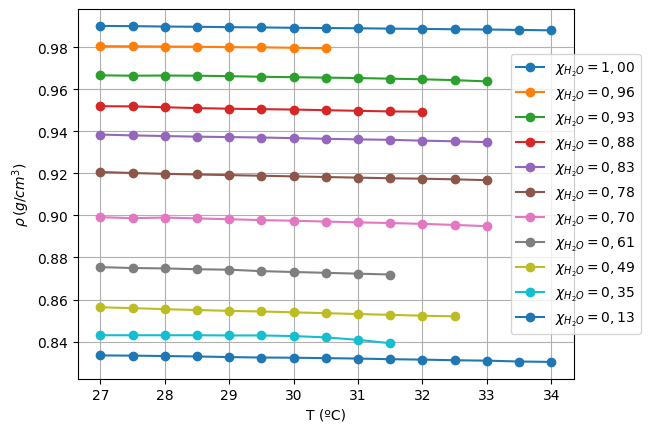
\includegraphics[width=0.85\linewidth]{Densidad/rho-T.png}
    \caption{Datos experimentales de $\rho(\chi,T)$}
    \label{fig:enter-label}
\end{figure}

\begin{equation}
    \begin{gathered}
        \rho(\chi) = 0,1999\chi^2 - 0,041\chi + 0,8344\\
        s(a) = 0,010 \; g\cdot cm^{-3} \quad s(b) = 0,013 \; g\cdot cm^{-3} \quad s(c)= 0,0034 \; g\cdot cm^{-3}
    \end{gathered}
\end{equation}

\begin{figure}[h!]
    \centering
    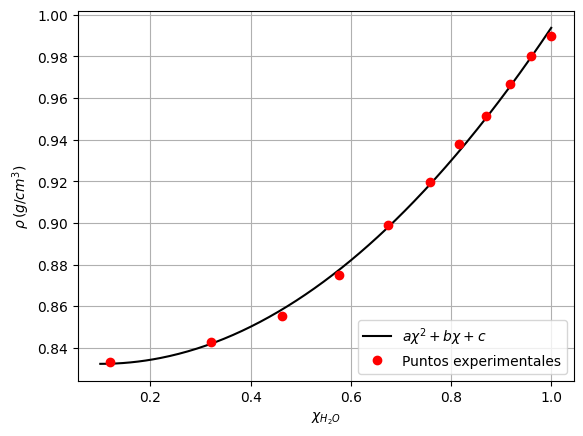
\includegraphics[width=0.85\linewidth]{Densidad/rho-x.png}
    \caption{$\rho(\chi) = 0,1999\chi^2 - 0,041\chi + 0,8344$}
    \label{fig:enter-label}
\end{figure}

\end{document}